\section{Case Study 1: Publication Data}
In this section, we demonstrate an application of TimeSets in analyzing publication data. We use a subset of 200 publications with the most citations from the IEEE InfoVis articles~\cite{Stasko2013}. Each publication includes one or many \emph{concepts} such as \emph{network} or \emph{evaluation}. We use this concept as the set attribute to group publications. Figure~\ref{fig:citations} shows the visualization of this dataset. No aggregation is needed when producing the layout; only complete and trimmed labels are used.

\begin{figure}[!htb]
\centering
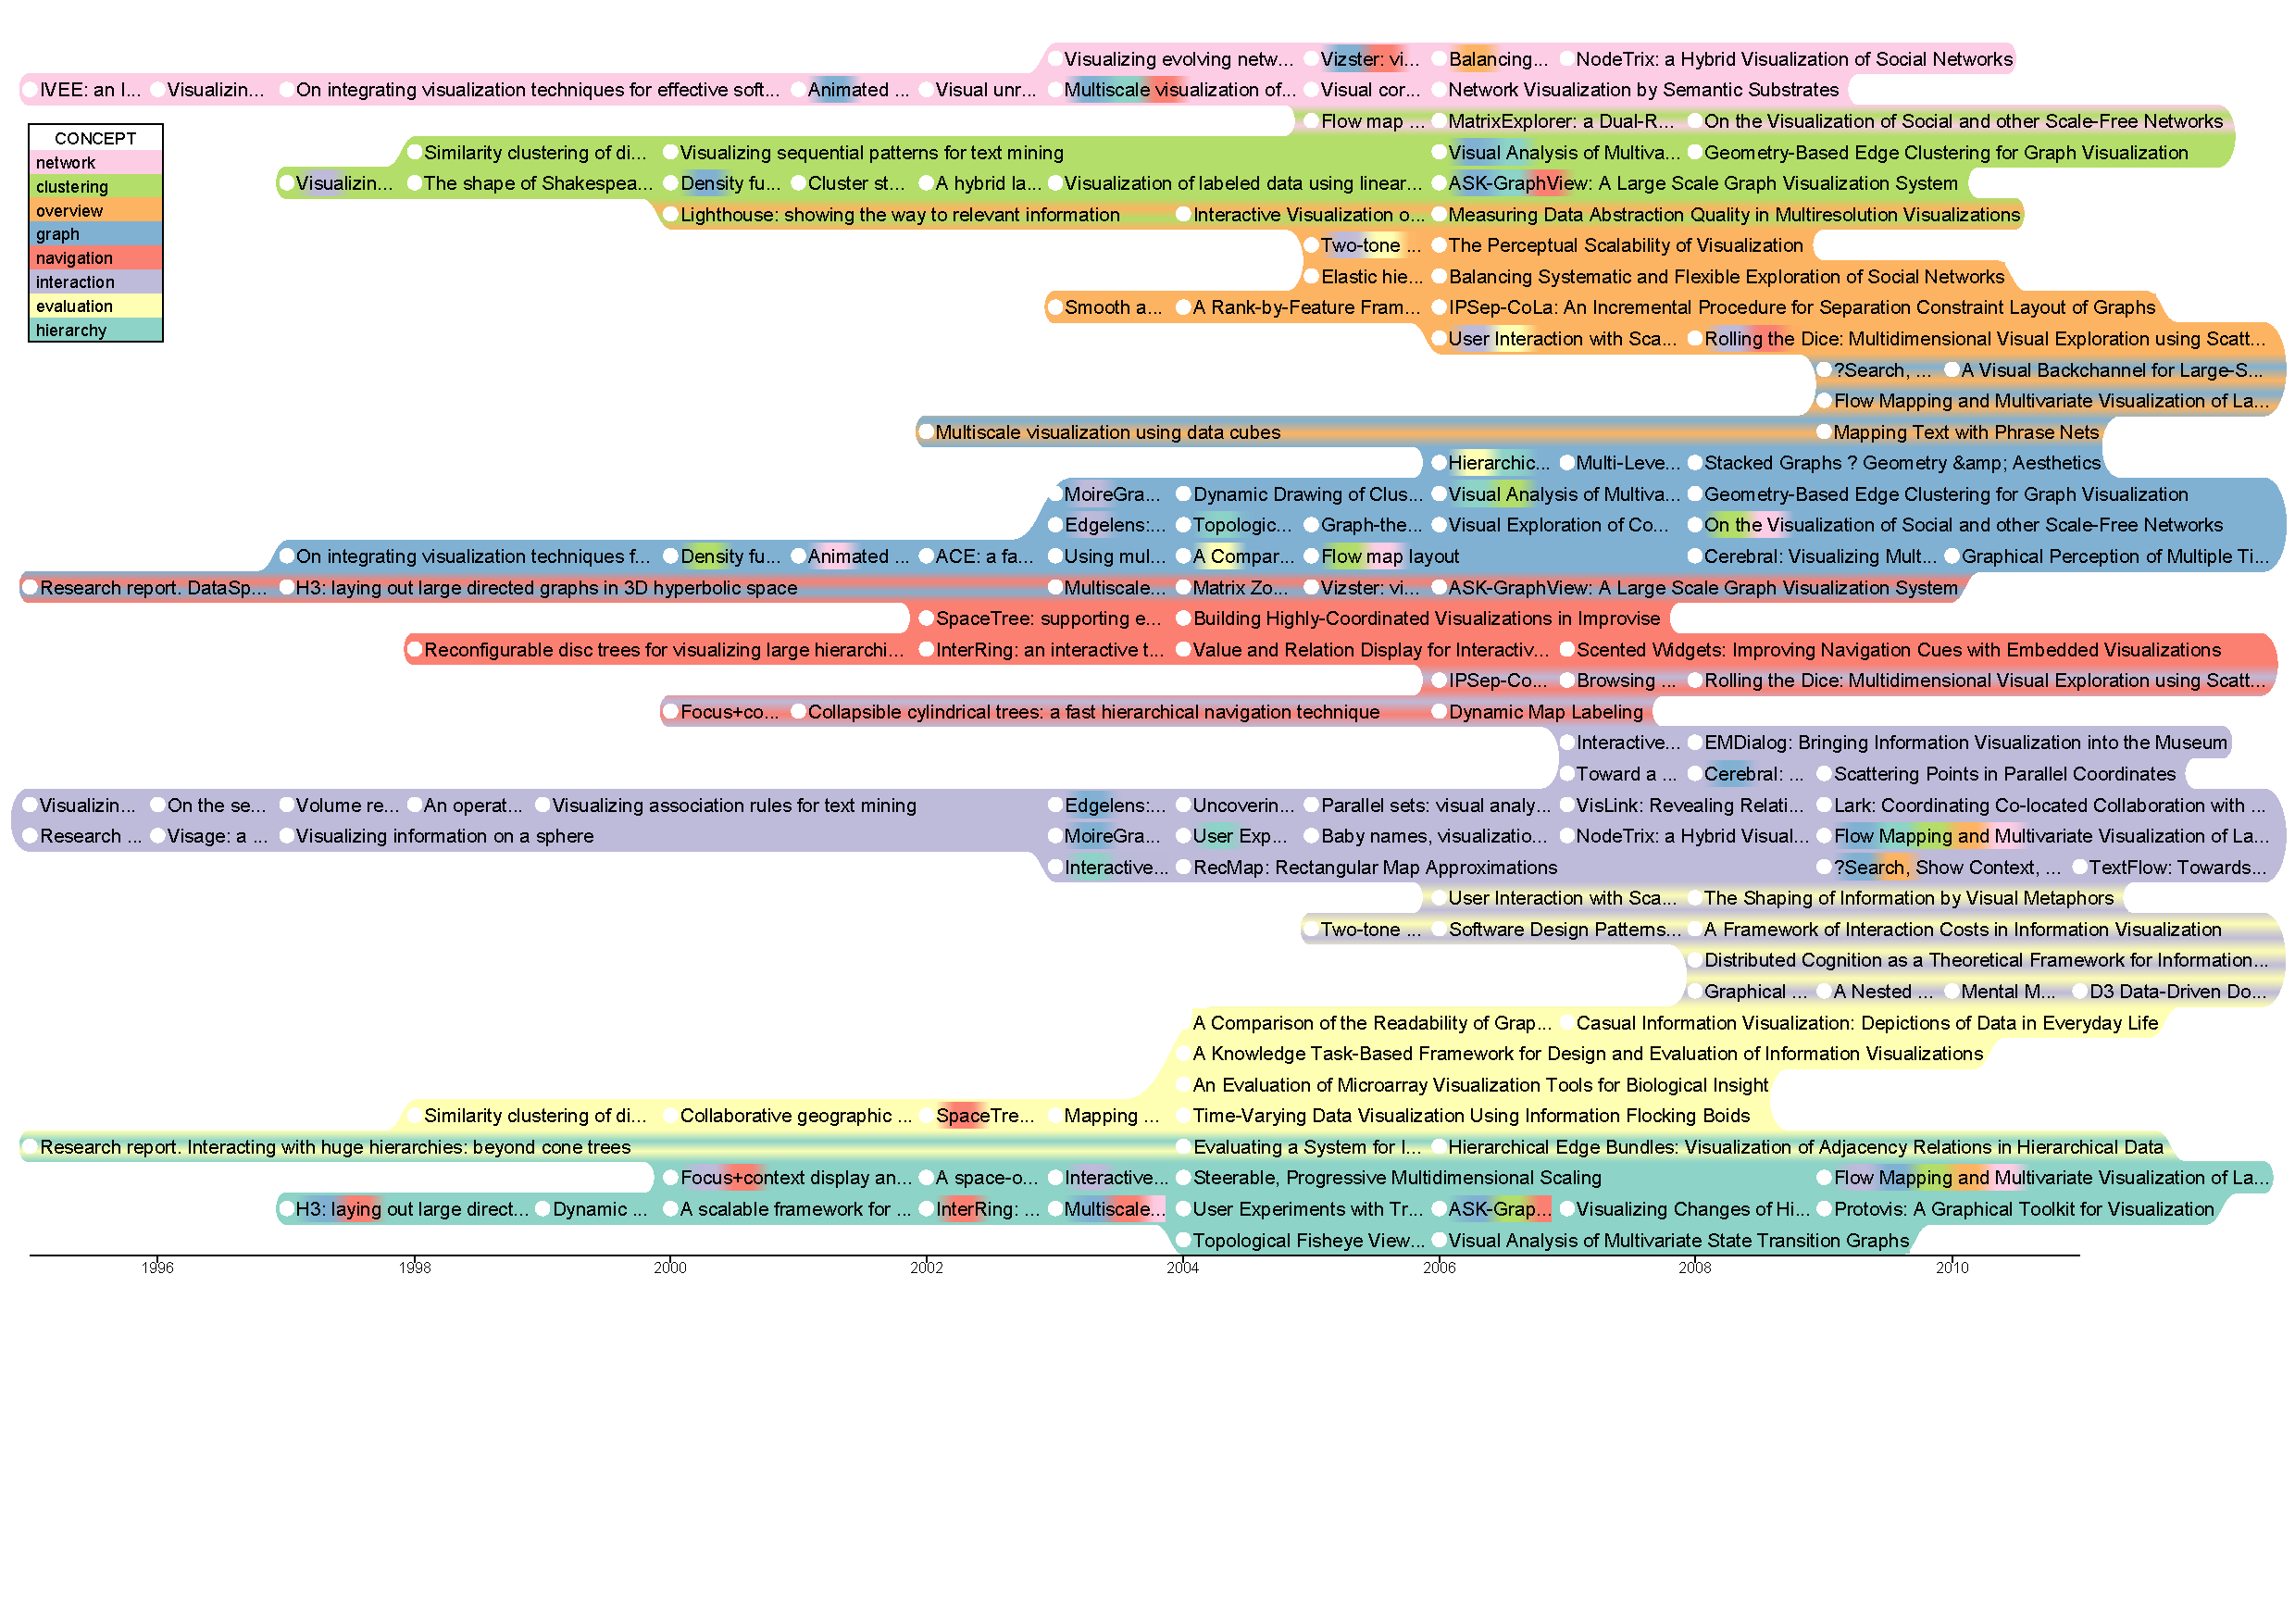
\includegraphics[width=\linewidth]{figure13}
\caption{TimeSets visualization of publication data. It shows 200 articles with the most citations in the IEEE InfoVis conference from 1995 to 2013. These articles are categorized based on their concepts (see the legend in the top left hand corner).}
\label{fig:citations}
\end{figure}

TimeSets can reveal the temporal distribution of thematic data as in ThemeRiver~\cite{Havre2002}. A quick glance at the visualization brings us a surprise. There is much void space on the left as opposed to a very dense area on the right indicating that there are many more highly cited papers published in the last ten years than those in the first ten years. This trend also holds for individual concepts: each colored layer starts with a single row and becomes higher towards the end of the timeline. This observation is in contrast with our thought: articles that have been published since longer time ago would receive more citations. One possible explanation is that the IEEE InfoVis conference has accepted more papers over time: in the dataset, 18 articles were published 1995, whereas 37 articles were published in 2013. Another reason could be that articles in the last ten years are really of higher quality.

TimeSets cannot show all intersections among sets; however,  its layout maximizes the number of shared elements between two neighboring sets. Therefore, the visible intersections usually include the most elements of all intersections. In the visualization, the most notable gradient area is the intersection between the yellow and the purple sets indicating that many excellent articles focus on both \tsevaluation{} and \tsinteraction. Also, at the top of the visualization, three concepts: \tsnetwork, \tsclustering{} and \tsoverview{} with ``clustering'' is in between the other two. This is expected because clustering techniques are important in visualizing large networks and providing an  overview of a large dataset.

In Figure~\ref{fig:citations}, TimeSets uses the color gradient method to show full memberships of multi-set elements. For instance, inside the \tsnetwork{} layer , there are quite a few small blue gradients for \tsgraph. This makes sense because the close relationship between these two concepts, and they may often appear together in the same articles. We also notice an article including the most concepts at the bottom of the visualization: ``Flow Mapping and Multivariate Visualization...'' (the last article on the third last row) with \tshierarchy, \tsinteraction, \tsgraph, \tsoverview{} and \tsnetwork.